\chapter{\MakeUppercase{Программная архитектура}}
\section{Структура управления}

\section{Протокол передачи данных} \label{sec:protocol}
Отправка команд от \textit{Raspberry Pi} к \textit{Arduino} и последующий прием обратной связи, производится через интерфейс \textit{Serial}. Это самый надежный вариант при условии, что для установки соединения используется обыкновенный \textit{USB} кабель, который уже защищен от помех и штекер которого надежно закреплен в разъеме.

Для достижения наилучшей скорости реакции микроконтроллера на команды был разработан специальный протокол передачи данных и написаны легковесные программные библиотеки. Для платформы \textit{Arduino} код написан на языке \textit{C++}, для микрокомпьютера \textit{Raspberry Pi} была разработана библиотека на языке \textit{Python}.

\noindent Библиотека для передачи данных написана для трёх платформ. Она сильно упрощает наладку управления \textit{Arduino} с помощью \textit{Raspberry Pi}. Основная идея программного кода в том, чтобы микрокомпьютер отправлял на микроконтроллер максимально простые команды, состоящие из массива байт, в который зашифрованы лишь целочисленный номер и вещественные аргументы. Обратная связь от микроконтроллера реализована в формате \textit{JSON}.

\begin{figure}[h]
    \centering
    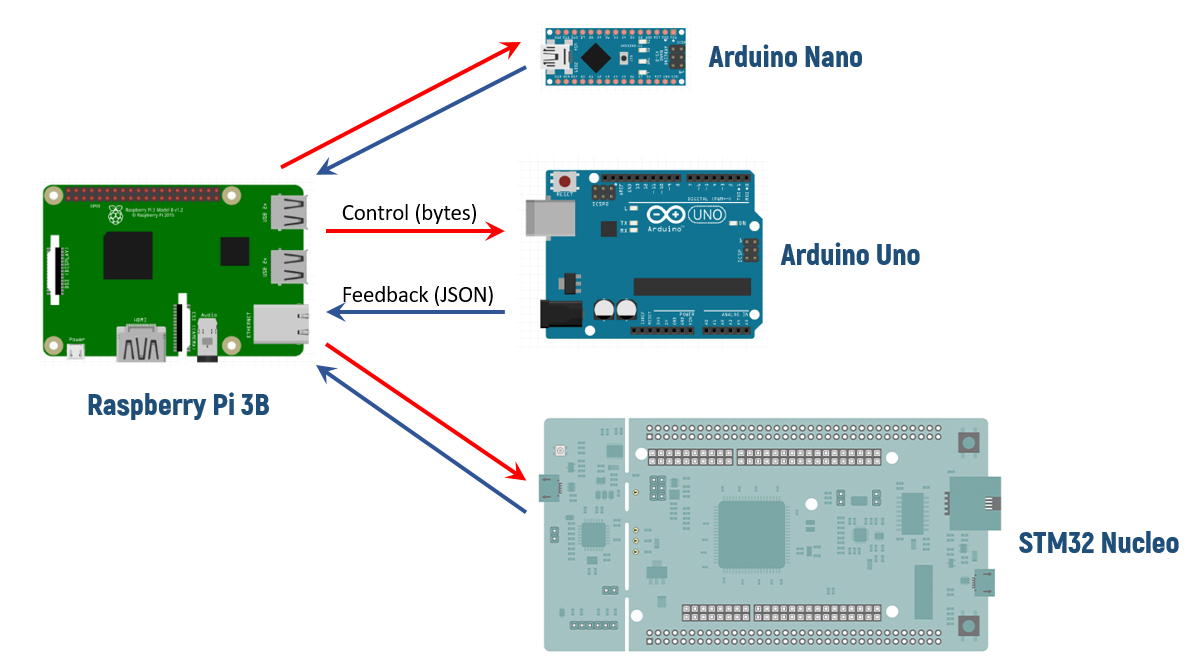
\includegraphics[scale=0.6]{chapter_arch/figure1.png}
    \caption{Управление микроконтроллерами с помощью \textit{Raspberry Pi}}
    \label{}
\end{figure}

\textbf{Для справки}: \textit{JSON} это сокращение от \textit{JavaScript Object Notation} -- формата передачи данных. Как можно понять из названия, {JSON} произошел из \textit{JavaScript}, но он доступен для использования на многих других языках, включая \textit{Python, Ruby, PHP} и \textit{Java}, в англоязычным странах его в основном произносят как \textit{Jason}, то есть как имя ДжЭйсон.Легкочитаемый и компактный, \textit{JSON} представляет собой хорошую альтернативу \textit{XML} и требует куда меньше форматирования контента.

\noindent Объект \textit{JSON} это набор данных в формате ключ-значение, который находится в фигурных скобках.
Вот так выглядит \textit{JSON} объект:
\begin{code}
{
  "first_name" : "Anton",
  "last_name" : "Kolomeytsev",
  "location" : "Moscow",
  "online" : true,
  "languages" : ["Russian", "English"] 
}
\end{code}

Преимущества выбранного подхода:
\begin{itemize}
    \item Микроконтроллер способен очень быстро расшифровать массив байт. Поэтому задержка между отправкой команды и её исполнением для человека не заметна.
    \item Невозможно перенести высокоуровневый функционал и принятие решений на микроконтроллер. И это хорошо.
    \item При таком формате общения между устройствами разработка  укладывается в основы теории автоматического управления.
    \item Возможность подключить до четырёх микроконтроллеров к одному \textit{Raspberry Pi}.
\end{itemize}

\textbf{Протокол}

Правила, по которым устанавливается соединение, следующие:
\begin{itemize}
    \item[1.] \textit{Raspberry Pi} устанавливает соединение с \textit{Arduino} по \textit{USB}, открывая \textit{Serial} порт между устройствами.
    \item[2.] \textit{Arduino} отправляет свой уникальный идентификатор.
    \item[3.] После получения идентификатора \textit{Raspberry} может использовать его для обмена данными. 
\end{itemize}

При написании кода на \textit{Raspberry}, есть всего три простых функции:

\noindent Функция \textit{push}: отправляет команду под номером \textit{CODE} с аргументами \textit{ARG}
\begin{code}
    clapi.device_id.push(CODE[, ARG1, ARG2, ..., ARGN])
\end{code}

\noindent Функция \textit{pull}: блокирует выполнение программы, дожидается входящего сообщения от устройства. Возвращает \textit{JSON}, который нам прислало устройство.
\begin{code}
    clapi.device_id.pull()
\end{code}

\noindent Функция \textit{request}: отправляет команду как \textit{push}, после чего дожидается ответа как \textit{pull}.
\begin{code}
    clapi.device_id.request(CODE[, ARG1, ARG2, ..., ARGN])
\end{code}

Первая версия кода библиотеки для управления была написана в 2019 году, использовалась <<в боевых условиях>> и достойно показала себя на робототехнических соревнованиях \textit{Eurobot}. С тех пор код был доработан, дополнительно протестирован и оптимизирован под новые нужды.


\section{Кинематические расчеты}

\section{Тестирование кода}

\section{Абстракция над вычислениями}
